\chapter{Reinforcement Learning for Surgical Tensioning}
Robotic surgical assistants (RSAs), such as Intuitive Surgical's da Vinci, facilitate precise minimally invasive surgery~\cite{veldkamp2005laparoscopic}. These robots currently operate under pure tele-operation control, but introducing assistive autonomy has potential to improve surgical training, assist surgeons, reduce fatigue, and facilitate tele-surgery.
For example, when cutting thin tissue with surgical scissors, a surgeon may use a second or even a third tool to pin down and fixture the tissue.
This technique, called tensioning (also called traction), adds additional constraints on the material to prevent deformations during the cutting from drastically changing the position of the desired cutting path.
The optimal direction and magnitude of the tensioning force changes as the cutting progresses, and these forces must adapt to any deformations that occur. 
However, practically, the surgeon's tensioning policy is often sub-optimal because: (1) surgeon can automatically manipulate only two of the tools at once leaving any third arm stationary, and (2) asymmetric multilateral tasks (arms doing different procedures) are known to be challenging without significant training with the tele-operative system.

Therefore, it would be beneficial to automatically synthesize tensioning policies to best assist an open loop cutting trajectory. The first challenge is modeling the dynamics of cutting and tensioning. One way to model deformable sheets is with a 3-dimensional mass-spring-damper network. A sheet is a planar graph of point masses connected by damped springs at edges. $k$ of the point masses are constrained to be fixed at a particular 3D location, i.e., they are tensioned, and the positions of the remaining masses is determined by the dynamics induced these constraints. At each time step, the constraint can be moved to a new location. Cutting is modeled by removing a single edge in the graph at each time-step.  For $k$ assistive arms, the optimization objective is to plan  sequence of $k$ movable boundary value constraints to maximize cutting accuracy.

This problem constitutes a highly non-convex optimal control problem, whether cutting accuracy is a non-convex objective that measures the symmetric difference between a perfectly cut contour and the actual cut. Furthermore, the underlying deformable manipulation system is also highly non-linear. 
Efficient policy search techniques are required if we want to effectively assist a human surgeon seamlessly during a procedure.
What is different about this problem is that we do not have access to ``expert demonstrations'' as in the previous chapters. 
Instead, we show that we can get an approximate suboptimal controller using physics-based approximations and then use Deep RL to fine-tune this controller. 
The archite

\section{Motivation}
Nienhuys and Van Der Stappen proposed the seminal work on modeling cutting with finite-element mesh models~\cite{nienhuys2001surgery}.
This work led to a bevy of follow-on work in robotics and graphics modeling the cutting problem, especially in the context of surgical simulation~\cite{bielser2004state, sifakis2007arbitrary, mendoza2003simulating, steinemann2006hybrid}.
In parallel, the graphics community studied fabric modeling with similar finite-element techniques~\cite{gale2016patterning, brookes16tearable}.
In our prior work, we implemented such an approach for the Pattern Cutting task in the Fundamentals of Laparoscopic Surgery (FLS)~\cite{thananjeyanmultilateral}.
This paper is inspired by the challenges noticed in our prior work, namely, that state-estimation of a deformable object when there are occlusions is very challenging. 
Therefore, we investigate whether synthesizing a tensioning plan \emph{a priori} can mitigate this problem.

Manipulation of deformable materials, particularly cutting, is a challenging area of research interest in robotic surgery \cite{nienhuys2001surgery, murali2015learning} as well as in computer graphics and computational geometry \cite{zhang2004cutting,Chentanez2009}. The use of expert demonstrations has been considered in prior work as an alternative to explicit models and simulations when studying and handling deformations in the environment. For example, Van den Berg et al. \cite{vandenBerg2010}, Osa et al. \cite{Osa2014}, and Schulman et al. \cite{Schulman2013} all approached manipulation of suture material using Learning From Demonstrations (LfD), an approach that uses demonstration trajectories to learn how to execute specific tasks.
RL has been a popular control method in robotics when dynamics are unknown or uncertain \cite{kober2013reinforcement}.
There are a few examples of RL applied to deformable object manipulation, e.g. folding \cite{balaguer2011combining} and making pancakes \cite{beetz2011robotic}.
The recent marriage between RL and Neural Networks (Deep RL)  opened a number of new opportunities for control in non-linear dynamical systems \cite{levine2015end}.
An obstacle to applying Deep RL to physical robots is that large amounts  of data are required for training, which makes sufficient collection difficult if not impossible using physical robotic systems--leading to our study of simulation-based learning.

\begin{figure}[t]
\centering
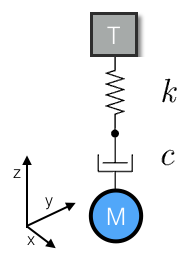
\includegraphics[width=0.32\textwidth]{tps-experiments/msd-1.png}
\caption{This illustration describes a basic mass-spring-damper system with spring constant $k$ and damping constant $c$. \label{illus:1}}
\end{figure}

\section{Physics of Multi-Dimensional Spring Systems}
As an introduction, we first describe the physics of a multi-dimensional spring system. This will provide the basic intuition for the deformable sheet model in the next section.
Figure \ref{illus:1} illustrates the most basic multi-dimensional spring system. A point mass $m$ is connected by a spring and damper to a infinitely strong block $T$. The spring constant is $k$ (let $\ell$ denote the resting length) and the damping constant is $c$. Let denote the acceleration vector $\mathbf{a} =  [ \ddot{x} ~~ \ddot{y} ~~ \ddot{z} ]^T$ of the point mass: 
\[
m \mathbf{a} = F_{spring} + F_{damper}.
\]
Hooke's law states that the magnitude of the force applied by a spring is proportional to its deviation $D$ from the rest length:
\[
|F_{spring}| = k D .
\]
Using unit vector notation, we can parametrize the force vector with spherical coordinates:
\[
F_{spring} =  ~\mathbf{i}~ k (D - \ell) \sin \theta \cos \psi +  ~\mathbf{j}~ k (D - \ell) \sin \theta \sin \psi + ~ \mathbf{k}~ k (D - \ell) \cos \theta 
\]
where $D = \sqrt{ (x-T_x)^2 + (y-T_y)^2 + (z-T_z)^2} $, $\theta = \cos^{-1} \frac{(z - T_z) }{D} $, $\psi = \tan ^{-1} \frac{(y - T_y) }{(x - T_x)}$.
For the damper, let $\mathbf{v} =  [ \dot{x} ~~ \dot{y} ~~ \dot{z} ]^T$ denote the velocity vector:
\[ F_{damper} = c \mathbf{v} .\]
The resulting equations of motion are:
\begin{equation}\footnotesize \selectfont
   m \mathbf{a} = ~\mathbf{i}~ (k (D - \ell) \sin \theta \cos \psi + c \mathbf{v}_x) +  ~\mathbf{j}~ (k (D - \ell) \sin \theta \sin \psi + c \mathbf{v}_y) + ~ \mathbf{k}~ (k (D - \ell) \cos \theta + c \mathbf{v}_z).
\end{equation}



\subsection*{Simulator}
We can use this model to design a simulator for cutting deformable sheets.
Let $G_{x,y,z} \subset \mathbf{R}^3 $ be a three-dimensional global coordinate frame. 
We denote the set of points on this sheet as $\Sigma$, and $\Sigma^{(G)}$ is the locations of these points in the global frame.
The points are connected by a graph of springs and dampers.
To apply the above equation of motion, we can treat each neighboring vertex as a wall.
For each $p \in \Sigma$, the neighboring vertex $q \in N(p)$ applies a force $F_{pq}$. 
Cutting is modeled as removing an edge from the graph.
In this paper, we assume that all of the springs have the same constant, natural length, and all the damping constants are the same.

The simulator is initialized with some initial state $\Sigma^{(G)}_0 \in G_{x,y,z}$. 
The state is then iteratively updated based on the derived equations of motion above.
For each $p \in \Sigma$, the updates have the following form:
%Interaction between the vertices is governed by:
\begin{align}
\label{eq:vertex}
m \ddot{p}  = \sum_{q \in N(p)} F_{pq} + F_{external}
\end{align}
To update the position $p$, we use the implicit Adams method with a standard python toolkit \footnote{https://docs.scipy.org/doc/scipy-0.14.0/reference/generated/scipy.integrate.ode.html}. Tensioning is simulated as a position constraint for a chosen pinch point $p' \in \Sigma$:
\[
p' = u
\]
This means that regardless of the forces applied to this point it will remain at position $u$.

\subsection*{Manipulation Actions}
We are given a rectangular planar sheet and a simple algebraic desired cutting contour of bounded curvature, which can be either closed or open.

\subsubsection{Cutting}
We assume that one arm of the robot is designated as the cutting arm and the other as the tensioning arm. A cutting contour is a sequence of points $C$ on the surface of the sheet. The cutting arm operates in an open-loop trajectory that attempts to cut along $C_0$, the position of the cutting contour in the global frame at time zero.
Error is measured using the symmetric difference between the desired contour on the sheet and the achieved contour cut. These will be different due to deformation of the sheet during cutting.
Let $X$ be the set of points inside a closed intended trajectory and let $Y$ be the set of points inside a closed simulated trajectory. The symmetric difference is then the exclusive-or $A \oplus B$ of the two sets. For open contours, the contours are closed by forming boundaries with the edges of the sheet.

\subsubsection{Tensioning}
Since the cutting is open-loop it cannot account for deformation, and this is why we need tensioning to apply feedback based on the state of the sheet.

\begin{definition}[Tensioning]
Let $s \in \Sigma$ be called a pinch point. 
Tensioning is defined as constraining the position of this pinch point to a specific location $u \in G_{x,y,z}$:
\[
T = \langle s, u \rangle
\]
\end{definition}

For each of the $k$ tensioning arms of the robot, we can have one tuple $T_i$. We consider a single pinch point for each arm for an entire cutting trajectory. This allows us to define a tensioning policy:

\begin{definition}[Tensioning Policy]
For arm $i\in \{1,..,k\}$, let $\Sigma^{(G)}_t$ be the locations of all of the points on the sheet in the global coordinate frame at time $t$. For a fixed pinch point $s$, a tensioning policy $\pi_s$ is a function where $\Delta_u = u_{t+1} - u_{t}$:
\[
\pi_i: \Sigma^{(G)}(t) \mapsto \Delta_u
\]

\end{definition}

\vspace{0.5em} \noindent\emph{Problem. Tensioning Policy Search: } For each arm $i$, find a tensioning policy that minimizes the symmetric difference of the desired vs. actual contour. 

\section{Reinforcement Learning For Policy Search}
We chose an RL algorithm since the symmetric difference reward function is non-convex and the system in non-linear.
We model the tensioning problem as a Markov Decision Process (MDP):
\[
\langle S,A,\xi(\cdot,\cdot), R(\cdot,\cdot),T \rangle.
\]
where the actions $A$ are 1$mm$ movements of the tensioning arm in the $x$ and $y$ directions, and the states $S$ are described below. The action space is tuned so the policy can generate sufficient tension to manipulate the cloth significantly over a few timesteps.  
Reward is measured using the symmetric difference between the desired contour and the achieved contour cut.
The robot receives 0 reward at all time-steps prior to the last step, and at the last time-step $T-1$ receives the symmetric difference. We do not shape the reward, as symmetric difference is exactly the error metric used for evaluation as well.

To optimize $\theta$, we leverage the TRPO implementation \cite{schulman2015trust} in Rllab \cite{duan2016benchmarking}. 
We use a neural network to parametrize the policy $\pi_\theta$, which maps an observation vector to a discrete action.
A two 32x32 Hidden Layer Multi-Layer Perceptron is used to represent this mapping. Since neural networks are differentiable, we can optimize the quantity $R(\theta)$.
The state space is a tuple consisting of the time index of the trajectory $t$, the displacement vector from the original pinch point $u_t$, and the location $x_i \in \mathbb{R}^3$ of fiducial points chosen randomly on the surface of the sheet. In all experiments we use $12$ fiducial points. 
This is a sample-based approximation of tracking $\Sigma^{(G)}_t$.


\section{Approximate Solution}
Directly applying the RL algorithm to the FEM simulator has a two problems: (1) large sample complexity and (2) local minima.
Even in an optimized simulator, every new contour required 5 minutes of learning before a viable policy was found.
The key insight was that ultimately the simulator used in RL was based on an analytic model.
Thus, we explored whether we could initialize learning with a prior developed from a simplified objective.

\subsection*{Small Deviation Approximation}
The equation of motion defines a non-linear system. We are, however, modeling point masses on a sheet that will have relatively small deformations from the resting length. 
We further assume that there is no damping $c=0$ or external forces.
For linearization, it is more convenient to work in Cartesian coordinates, so we can also re-parametrize the equations using Pythagorean identities:
\[
m a_x = k  \Delta_x - k \frac{\ell \Delta_x }{\sqrt{\Delta_x^2 + \Delta_y^2 + \Delta_z^2}} 
\]
\[
m a_y = k  \Delta_y - k \frac{\ell \Delta_y }{\sqrt{\Delta_x^2 + \Delta_y^2 + \Delta_z^2}}  
\]
\[
m a_z = k  \Delta_z - k\frac{\ell \Delta_z }{\sqrt{\Delta_x^2 + \Delta_y^2 + \Delta_z^2}} 
\]

To linearize, we can first take the gradient:
\[
\nabla(m a_x) = k \begin{bmatrix}
    1 - \frac{\ell (\Delta_y^2 + \Delta_z^2) }{(\sqrt{\Delta_x^2 + \Delta_y^2 + \Delta_z^2}) ^\frac{3}{2}} \\
    \frac{\ell \Delta_x \Delta_y }{(\sqrt{\Delta_x^2 + \Delta_y^2 + \Delta_z^2}) ^\frac{3}{2}} \\
    \frac{\ell \Delta_x \Delta_z }{(\sqrt{\Delta_x^2 + \Delta_y^2 + \Delta_z^2}) ^\frac{3}{2}} \\
\end{bmatrix} 
\]
We linearize around the operating point $\Delta_x, \Delta_y,\Delta_z = \rho = \frac{\ell}{\sqrt{3}}$, and let $\lambda = \frac{1}{3}\ell^{\frac{3}{2}}$:
\[
m a_x \approx  k \begin{bmatrix}
    1 - 2 \lambda \\
    \lambda \\
    \lambda \\
\end{bmatrix}^T \cdot \begin{bmatrix}
    (\Delta_x - \rho) \\
    (\Delta_y - \rho)\\
    (\Delta_z - \rho) \\
\end{bmatrix}, m a_y \approx  k \begin{bmatrix}
    \lambda \\
    1-2\lambda \\
    \lambda \\
\end{bmatrix}^T \cdot \begin{bmatrix}
    (\Delta_x - \rho) \\
    (\Delta_y - \rho)\\
    (\Delta_z - \rho) \\
\end{bmatrix}, m a_z \approx  k \begin{bmatrix}
    \lambda \\
    \lambda \\
    1-2\lambda \\
\end{bmatrix}^T \cdot \begin{bmatrix}
    (\Delta_x - \rho) \\
    (\Delta_y - \rho)\\
    (\Delta_z - \rho) \\
\end{bmatrix}
\]
We can define some notation to make the future algebra more concise:
\[
\mathbf{L} = \frac{k}{m} \begin{bmatrix}
   1- 2\lambda & \lambda & \lambda  \\
    \lambda & 1- 2\lambda & \lambda \\
    \lambda & \lambda  & 1-2\lambda \\
\end{bmatrix}
\]
The resulting system can be described in the state-space model for a position of a point mass $p$:
\begin{equation}
\ddot{p} = \mathbf{L} (\sum_{q \in N(p) }  (p - q) - \rho)
\end{equation}

\subsection*{Tensioning Problem}
The key trick to understanding tensioning based on this linearization is an efficient computation of the equilibrium state, i.e., $\ddot{p} = 0$.
Let $X \in \mathbb{R}^{N \times 3}$ denote the positional state of each of the masses.
For $N$ masses and $E$ edges, let $A$ be an $E \times N$ matrix where every $A_{ij} = 0$ if edge i is not incident to the mass $j$, $A_{ij} = \pm 1$ for edges incident to the mass (pushing or pulling, can be selected arbitrarily).
And, finally, let $R$ be an $\mathbb{R}^{E \times 3}$ matrix where each component is $\rho$, or the natural length of the spring.
It can be shown that the acceleration of all of the masses is:
\[
\ddot{\mathbf{P}} =  A^T A X L - A^T R L 
\]
making the equilibrium condition:
\[
 A^T A X  =  A^T R 
\]

To enforce constraints, we simply have to enforce that some subset of the components of $X$ are fixed.
This restricts the equilibrium solution to the subspace of values for which $X_{i,:} = u_i$.
These are exactly the tensioning constraints, and we can solve the system of equations by partitioning the masses into free and tensioned sets.

First, we can re-write the above equation as:
\[
B X =  A^T R
\]
which can in turn be written as:
\[
B_{free} X_{free}  = A^T R + B_{tens} U
\]
and solving for the least squares solution
\[
X_{free}  = (B_{free}^T B_{free})^{-1} [B_{free}^T A^T R + B_{free}^T B_{tens} U]
\]
This expression is just an affine function of the tensioning constraints:
\[
X_{free}  = C U + D
\]

\begin{figure*}[t]
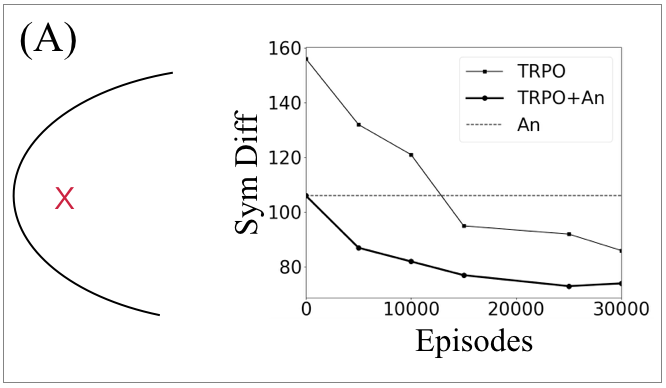
\includegraphics[width=0.32\textwidth]{tps-experiments/trpo-full-a.png}
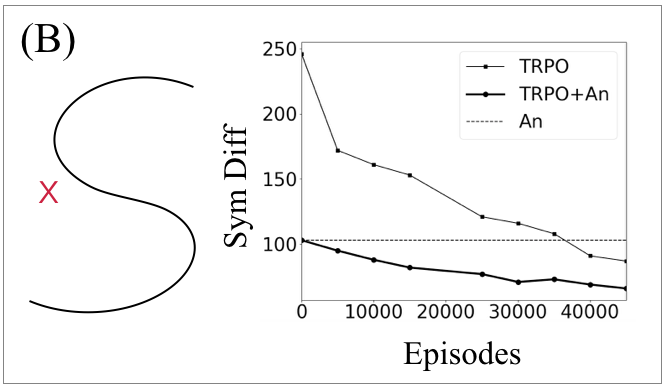
\includegraphics[width=0.32\textwidth]{tps-experiments/trpo-full-b.png}
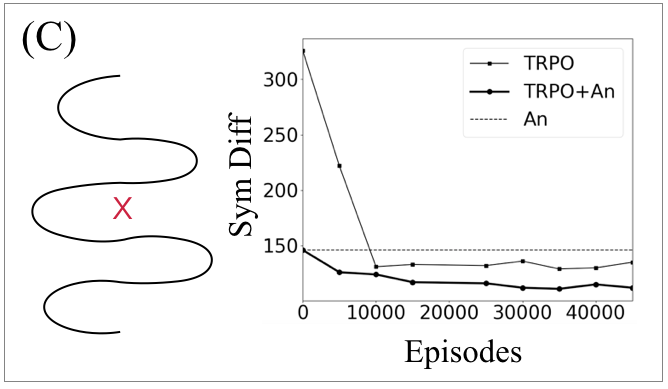
\includegraphics[width=0.32\textwidth]{tps-experiments/trpo-full-c.png}
\caption{This plot shows the expected reward over 50 trials for TRPO, TRPO initialized with the analytic approximation (TRPO AN), and the analytic model on its own. Three cutting curves are visualized of increasing difficulty with a single pinch point marked in red. Results suggest that initializing with an analytic model can greatly accelerate learning.\label{fig:1}}
\end{figure*}

\subsection*{Optimization}
To find tensioning directions and magnitudes, we have to pose an optimization problem to set the values of U as the grid is cut.
The model and its equilibrium states give us a way to quantify deformation induced by cutting.
$C$ and $D$ depend on the structure of the graph at time $t$.

We cannot directly optimize for symmetric difference so instead, we optimize for minimizing total deformation from the original state:
\[ I_{t} =  \| X_{free}[0] - X_{free}[t+1] \|^2_2 \]
This measures the amount of change in the position of the points after a cut and the sheet has settled into a new equilibrium state.
This sets up our control objective for synthesizing a set of tensions from a fixed pinch point. 
\begin{equation}
   \min_{u_1,...,u_T} \sum_{t=0}^{T-1} I_{t} + q \|u_{t+1} - u_t \|_2^2  \label{obj}
\end{equation}
where $q \|u_{t+1} - u_t \|^2_2$ is a control penalty on changing the tensioning between time-steps for $q > 0$. 


This problem is a convex program which can be solved with standard solvers.
Once this open-loop strategy is learned, we can initialize TRPO by training the policy network to predict $u_{t}$ from the state.
Out intuition is that this analytic model gets close to the optimal policy and TRPO simply has to refine it.
This mitigates the effects of bad local minima far from the optimum and slow convergence.

\section{Experiments}

\subsection*{Performance}
We present a set of illustrative initial experiments in this paper.
In the first experiment, we generated three contours of increasing difficulty and learned tensioning policies for a single pinch point $k=1$.
We compare TRPO with no initialization, TPRO+An with the analytic initialization, and An which is just the analytic model.
Figure \ref{fig:1} plots the learning curves.
We stopped training when the reward was no longer reliably decreasing.
We find that in all three cases, the analytic initialization significantly reduces the time needed to learn a similarly successful policy.
Furthermore, the analytic model is within 25\% of the final reward of TRPO achieves indicating that it is a very good initialization.

The next experiment evaluates the run time of the algorithms as we increase the number of tensioning arms.
Figure \ref{fig:2}A measures the number of episodes needed for TRPO to crossover, i.e., match the performance of the analytic method, as a function of the number of tensioning arms to plan for.
While the analytic method is greedy, TRPO requires nearly 350000 episodes before it is at parity with this method for 4 tensioning arms.
For comparison, the analytic optimization requires two orders of magnitude less time to reach the same result (Figure \ref{fig:2}B).
And, we explore using the combination of the two to achieve higher accuracy results with less rollouts.

\begin{figure}[ht]
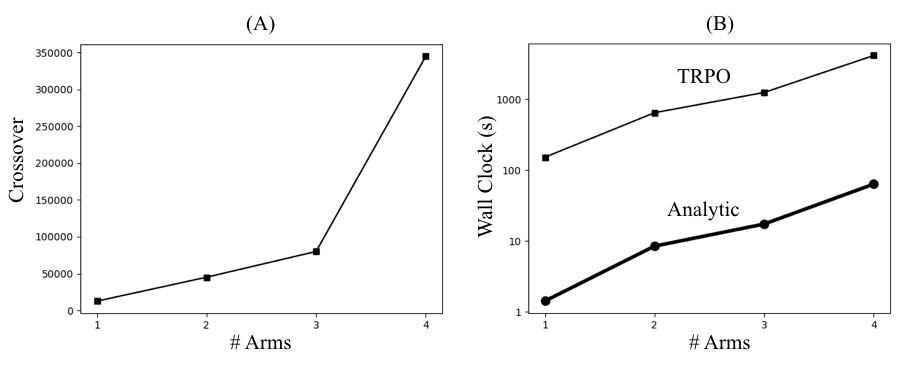
\includegraphics[width=\columnwidth]{tps-experiments/trpo-6.png}
\caption{(A) We measure the number of episodes needed for TRPO to crossover, i.e., match the performance of the analytic method, as a function of the number of tensioning arms to plan for. (B) For comparison, we plot the wall clock time of TRPO and the analytic optimization on a log scale. The optimization is order of magnitudes faster, but may be suboptimal. \label{fig:2}}
\end{figure}

\subsection*{End-to-End}
\newcommand{\shapesize}{0.75}
\begin{table}[t]
\centering
\caption{\textbf{Evaluation of \tpsalgo}: For the 17 contours shown, we evaluate the three tensioning policies described in \secref{policyeval}.  We measure and report performance in terms of relative percentage improvement in symmetric difference over a baseline of no tensioning for the tensioning trials. The 95\% confidence interval for 10 simulated trials is shown for fixed, analytic, and Deep RL tensioning, while the mean absolute symmetric difference error is reported for the no-tensioning baseline experiments.
%The formula to compute this is $100 \times \frac{\text{score}_i - \text{score}_j}{\text{score}_j}$, where $i \in$ \{fixed, analytic, Deep RL\} and $j=$no-tensioned.
The data suggest that \tpsalgo  performs significantly better in comparison to the fixed and analytic baseline. The corresponding pinch points used for fixed and \tpsalgo  are indicated in red. The analytic pinch point is the centroid of the shape.}
\resizebox{\linewidth}{!}{% put in textwidth
\begin{tabular}{llcccc}
% \toprule
\hline
&\textbf{Shape} & \multicolumn{4}{c}{\textbf{Tensioning Method}} \\
& & \multicolumn{1}{c}{\textbf{No-Tension}} & \multicolumn{1}{c}{\textbf{Fixed}} & \multicolumn{1}{c}{\textbf{Analytic}} & \multicolumn{1}{c}{\textbf{Deep RL}} \\
% \midrule
\hline  \hline
1  &  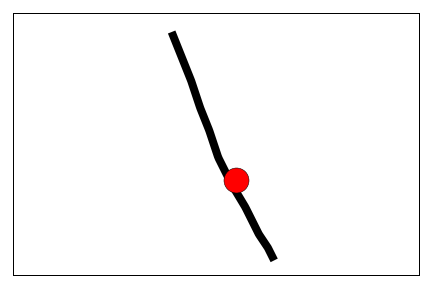
\includegraphics[height= \shapesize cm]{tps-experiments/shapes/pts_21.png} &        17.4 &          -20.69$\pm$4.44 &        -149.43$\pm$10.24 &  \textbf{64.37$\pm$5.77} \\
2  &  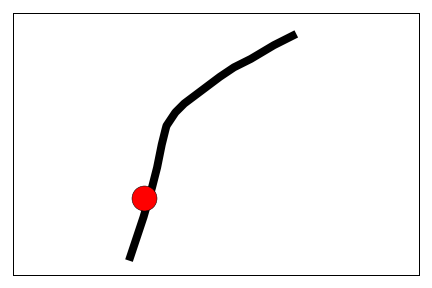
\includegraphics[height= \shapesize cm]{tps-experiments/shapes/pts_20.png} &        22.5 &           32.44$\pm$1.74 &         -117.78$\pm$0.00 &  \textbf{55.11$\pm$7.40} \\
3  &  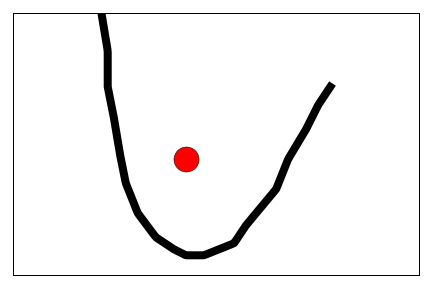
\includegraphics[height= \shapesize cm]{tps-experiments/shapes/pts_12.png} &        23.2 &          -21.12$\pm$5.41 &           18.10$\pm$1.78 &  \textbf{38.36$\pm$9.43} \\
4  &  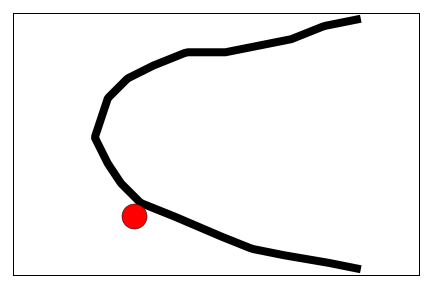
\includegraphics[height= \shapesize cm]{tps-experiments/shapes/pts_11.png} &       102.9 &            7.48$\pm$0.62 &           30.42$\pm$1.45 &  \textbf{36.15$\pm$3.97} \\
5  &  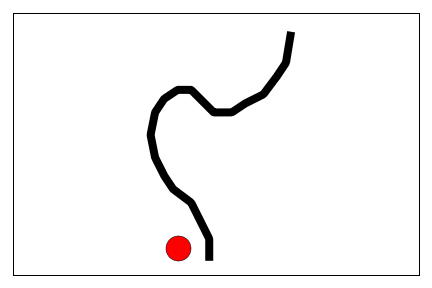
\includegraphics[height= \shapesize cm]{tps-experiments/shapes/pts_17.png} &        41.1 &            0.49$\pm$7.99 &            9.98$\pm$0.00 &  \textbf{52.31$\pm$7.26} \\
6  &  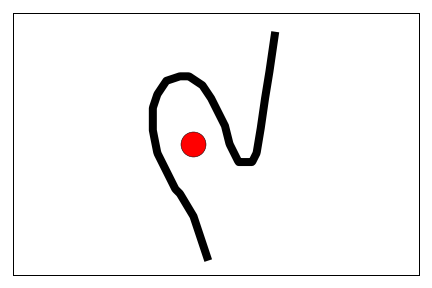
\includegraphics[height= \shapesize cm]{tps-experiments/shapes/pts_18.png} &        42.0 &  \textbf{55.00$\pm$1.77} &           11.43$\pm$1.52 &           45.95$\pm$6.60 \\
7  &  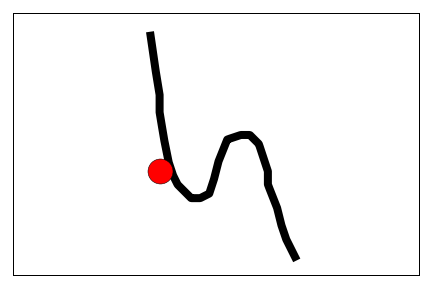
\includegraphics[height= \shapesize cm]{tps-experiments/shapes/pts_19.png} &        40.2 &           22.64$\pm$1.14 &            3.73$\pm$1.46 &  \textbf{33.83$\pm$3.99} \\
8  &  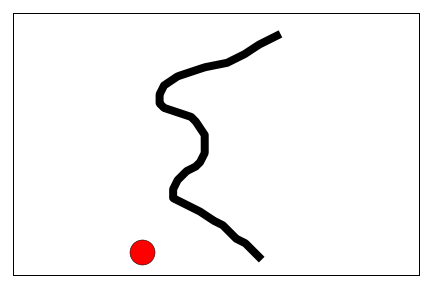
\includegraphics[height= \shapesize cm]{tps-experiments/shapes/pts_16.png} &        40.0 &           -1.25$\pm$0.82 &            1.75$\pm$2.83 &  \textbf{35.50$\pm$4.67} \\
9  &  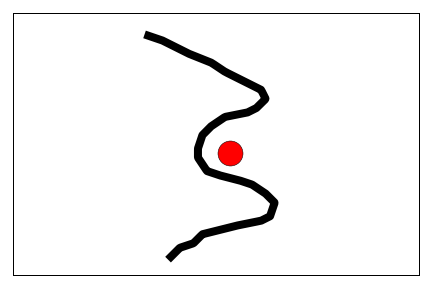
\includegraphics[height= \shapesize cm]{tps-experiments/shapes/pts_14.png} &        66.6 &            2.85$\pm$2.60 &  \textbf{34.68$\pm$2.25} &           28.38$\pm$4.98 \\
10 &   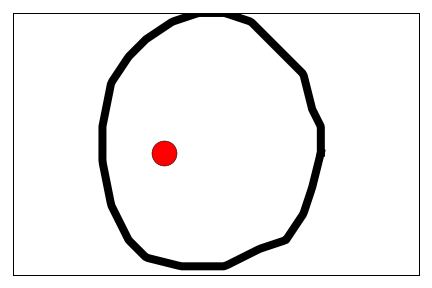
\includegraphics[height= \shapesize cm]{tps-experiments/shapes/pts_1.png} &        63.6 &           25.63$\pm$2.98 &           20.60$\pm$3.60 &  \textbf{41.35$\pm$9.90} \\
11 &   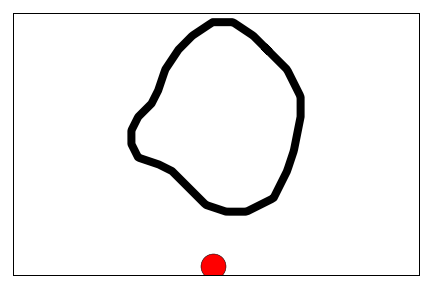
\includegraphics[height= \shapesize cm]{tps-experiments/shapes/pts_9.png} &        73.6 &            2.31$\pm$1.66 &           24.32$\pm$0.98 &  \textbf{56.11$\pm$8.99} \\
12 &  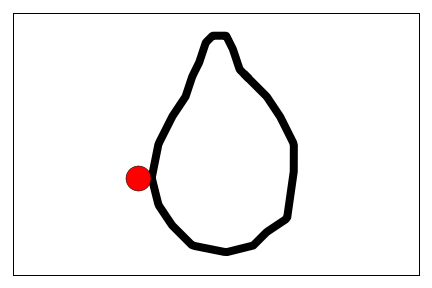
\includegraphics[height= \shapesize cm]{tps-experiments/shapes/pts_10.png} &        79.3 &           22.82$\pm$4.51 &           55.49$\pm$0.38 &  \textbf{63.56$\pm$3.61} \\
13 &   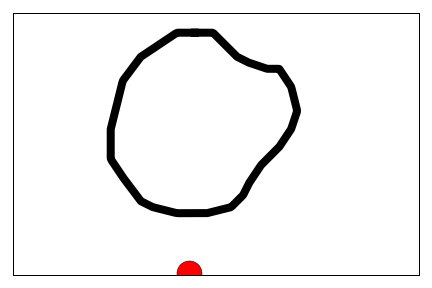
\includegraphics[height= \shapesize cm]{tps-experiments/shapes/pts_8.png} &        94.3 &            3.29$\pm$2.05 &           27.15$\pm$0.32 &  \textbf{34.04$\pm$5.87} \\
14 &   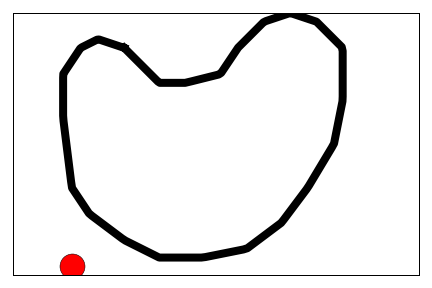
\includegraphics[height= \shapesize cm]{tps-experiments/shapes/pts_3.png} &        71.7 &            3.07$\pm$7.15 &           -2.51$\pm$0.61 &  \textbf{39.89$\pm$8.20} \\
15 &   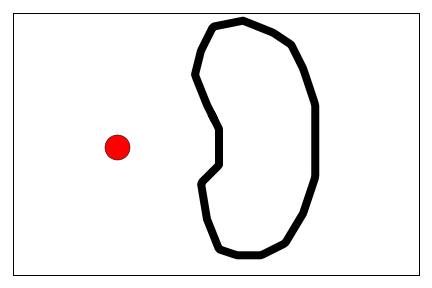
\includegraphics[height= \shapesize cm]{tps-experiments/shapes/pts_2.png} &       178.7 &           74.71$\pm$1.22 &           80.75$\pm$0.88 &  \textbf{81.25$\pm$1.38} \\
16 &   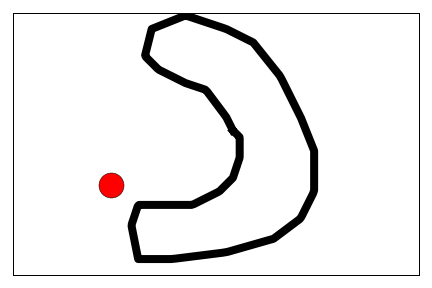
\includegraphics[height= \shapesize cm]{tps-experiments/shapes/pts_4.png} &       114.6 &           -8.03$\pm$2.16 &  \textbf{31.06$\pm$0.62} &           29.06$\pm$8.81 \\
17 &   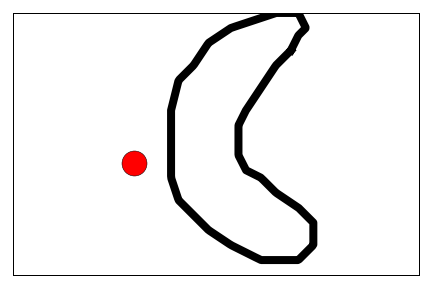
\includegraphics[height= \shapesize cm]{tps-experiments/shapes/pts_7.png} &        74.8 &           10.29$\pm$2.08 &  \textbf{28.34$\pm$2.07} &            0.80$\pm$7.03 \\
\hline 
\multicolumn{2}{c} { Mean (\%)} &  &13.54$\pm$9.84 &
9.70$\pm$21.96 & 
\textbf{43.30$\pm$8.61}  \\
\hline
% \hline
\end{tabular}
}
\vspace{-10pt}
\end{table}

% \begin{figure*}
% \vspace{-10pt}
%     \centering
%     \vspace{-5pt}
%     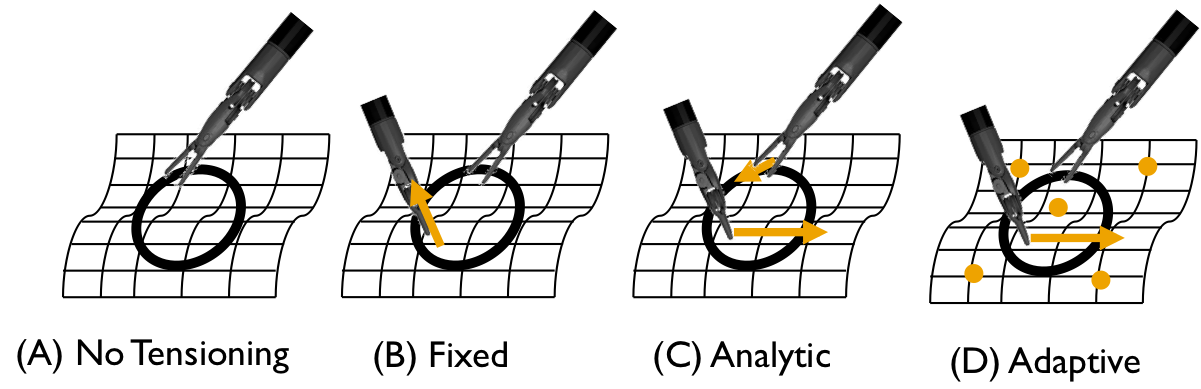
\includegraphics[width=\textwidth]{./tps-experiments/tensioning-algos.png}
%     \caption{A comparison of all of the tensioning policies. (A) No tensioning cuts the trajectory without using the tensioning arm, (B) Fixed Tensioning applies a fixed tension at a point, (C) Analytic applies a proportional control policy that observes the difference between the line and the cutting arm and applies tension proportional to the error and (D) Adaptive tensioning is the proposed approach that tracks the state of the gauze using fiducial points.  }
%     \figlabel{noise}
%     \vspace{-15pt}
% \end{figure*}
	
% \subsection*{Simulation Experiments}
% \subsubsection{\tpsfull}
Next, we compare \tpsalgo to alternative tensioning approaches.
We first evaluate the techniques in terms of performance by calculating the symmetric difference between the target pattern and actual cut.
Then, we compare the techniques in terms of robustness by tuning the techniques for one simulated parameter setting and then applying them to perturbations.

% \subsubsection{Evaluation of \tps}
\subsection*{Cutting Accuracy}
\label{sec:policyeval}
We manually drew 17 different closed and open contour to evaluation in simulation, as illustrated in the table. 
%\todo{do you do all experiments for all 21 shapes? if not, make this into an experiment section not as part of setup}
For each of the contours, we evaluated four different tensioning methods:
\begin{itemize}
\item \emph{Not Tensioned:} Single-arm cutting is performed with no assisted tensioning other than the stationary corner clips that fix the sheet in place.
\item \emph{Fixed Tensioning:} The material is pinched at a single point with the gripper arm (with corner points still fixed in place), but no directional tensioning is applied. We simulate area contact by pinching a circular disc.
\item \emph{Centroid Tensioning:} Tensioning is proportional to the direction and magnitude of the error in the  3D position of the cutting tool and the closest point on the desired contour. The gain was hand-tuned on randomly-chosen contours and is fixed to 0.01.
\item \emph{\tpsalgo }  A separate policy is trained for each shape, this requires 20 iterations of TRPO in the simulator.
\end{itemize}

\vspace{0.5em}

% More formally, let $X$ be the set of points inside a closed intended trajectory and let $Y$ be the set of points inside a closed simulated trajectory. The symmetric difference is then simply the exclusive-or $A \oplus B$ of the two sets. Open curves are treated as closed curves by forming boundaries with the edges of the cloth. \todo{ replace with image, cut, or condense into footnote. don't need to go into detail of SD}.
For the analytic tensioning model, the centroid of the contour is used as the pinch point. For the fixed policy, the point was chosen by random search over the feasible set of points.
Performance is measured using the symmetric difference between the desired contour and the actual cut.

The averaged symmetric difference scores for each instance  and tensioning method are reported in table.  
The success of the different tensioning algorithms are presented as the percentage of improvement in symmetric difference score over the non-tensioned baseline. 
The average of the scores over all 17 contours are also included in the table.   
For the selected set of contours, \tpsalgo achieves the best average relative improvement of $43.30\%$, the analytical method $9.70\%$, and the fixed approach $13.54\%$.
%{\footnotesize
%\begin{table}[h]
%\centering
%\begin{tabular}{ c c c }
%passive tension & analytic tension & learned tension\\
%\hline \hline%
%	$30.34 \pm% 2.00$\% & $10.12 \pm 7.66$\% & $43.26 \pm 2.94$\%
%\end{tabular}%}
%\caption{caption}\label{tab:average21}
%\end{table}

\subsection*{dVRK: Hardware and Software}
% \subsection*{dVRK: Hardware and Software}
We use the Intuitive Surgical da Vinci Research Kit (dVRK) surgical robot assistant, as in~\cite{murali2015learning,sen2015automating,garg2016gpas}. We interface with the dVRK using open-source electronics and software developed by~\cite{Kazanzides2014}. The software system is integrated with ROS and allows direct robot pose control.
We use the standard laparoscopic stereo camera for tracking fiducials on the surgical gauze. We equip the right arm with the curved scissors tooltip for cutting and the left arm with the needle driver tooltip for pinching and tensioning. The arms are located on either side of the surgical gauze to maximize the workspace for each without collision.
% \todo{from reviewer: The experimental setup is not described with enough details (for example which tools are used? how the slave arms are placed with respect to the camera? How did you solve the hand to hand and hand to eye problem?), probably a picture of the setup will help in the description.}
% \todo{picture of setup might be nice}
% \vspace{2pt}
\subsection*{Physical Evaluation of \tpsalgo} 
We show the physical results on 4 contours using Fixed Tensioning and Deep RL using the symmetric difference as the evaluation metric in table. The tensioning policy for Deep RL was derived from simulation experiments by registering the physical gauze to a sheet in the simulator environment. 
In this set of experiments, we used fixed tensioning as the baseline.
The no tensioning policy frequently failed in the physical experiment so we excluded that from the results table for a fair baseline comparison.
We were unable to evaluate the analytic method in the physical experiments because the state-estimation needed for feedback control was not possible outside of the simulated environment.

 We do not attempt analytic tensioning since it requires real-time tracking of the pattern to estimate local error. We observed that 3 out of 4 of the \tpsalgo experiments performed better than the fixed tensioning policy with respect to the symmetric difference of the cut and ideal trajectories. This is the same objective the trained policy was designed to minimize in simulation. A weakness of the policy was failure to address discrete failure modes, including discrete failure modes induced by the policy itself. Failure as a result of the scissors' entanglement in the gauze occurred in both experimental groups. The active manipulation and tensioning of \tpsalgo also caused increased deformation of the cloth which occasionally directly resulted in entanglement as well. We did not optimize our policy to minimize these discrete failures, and our simulator does not model the robot with acceptable fidelity to do so. To address this, we would require very accurate models of the robot arms and tools.
% \todo{From reviewer: The experimental evaluation is not well described, it is not clear the relations between simulated and real experiments, and how to compare the results from the two experiments.}
% \todo{From reviewer: Section VIII on physical experiments is unfortunately the
% weakest on the paper. Apart from the low number of
% experiments, it would have been useful for the reader to
% see at least a representative example of the kind of errors
% caused during real experiments by fixed and Deep RL
% tensioning. Having only a percentage improvement instead of
% an absolute metric in $mm^2$ makes it difficult to judge
% whether either method is acceptable, regardless of their
% relative performance w.r.t. one another. This would be
% useful especially given that the relative improvement
% between techniques oscillates wildly in both simulations
% and real experiments, so it is difficult for the reader to
% assess what is actually going on. Finally, physical
% experiments using the 17 patterns learnt during the
% simulations would have been useful to validate the relative
% performance shown during simulations.
% }
% We use an $8$\,mm Needle Driver with a PALP probe mounted on the gripper \cite{mckinley2015disposable}. 

% We selected curves \todo{U, V, X, Y, Z} shown in \tabref{scores-dvrk}. The results are summarized in \tabref{exp}. \figref{teaser} also illustrates the results in the case of \todo{}.

\begin{table}[t!]
\centering
\vspace{5pt}
\caption{\textbf{dVRK Physical Experiments}: This table compares the relative percentage improvement in terms of symmetric difference to a baseline of fixed tensioning to \tpsalgo in experiments performed on the dVRK robot. The black dot indicates the pinch point of the gripper arm.}
% \begin{tabular}{lll}
% % \begin{tabular}{>{\centering}m{0.1in} l >{\centering}m{.5in} >{\centering}m{.5in} >{\centering}m{.5in}}
% % \toprule
% \hline
% \rowcolor[HTML]{CBCEFB}
% %&Shape & Tensioning Method \\
% %\rowcolor[HTML]{CBCEFB}
% &  Shape & Deep RL \\
% % \midrule
% \hline  \hline
% 1  &  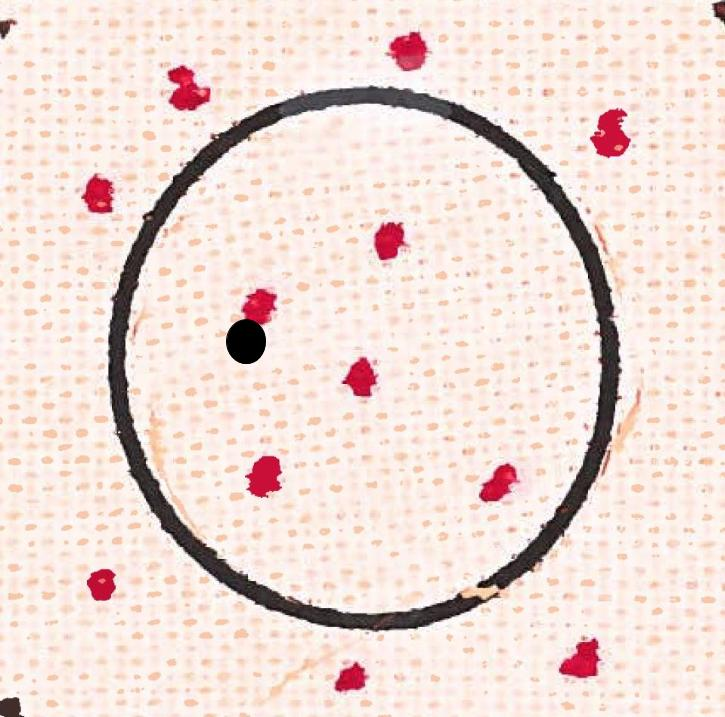
\includegraphics[height=1cm]{tps-experiments/shapes-robot/1-dot.jpg} &           \textbf{118.63 \%}
% \\
% \rowcolor[HTML]{E0E0E0}
% 2 &   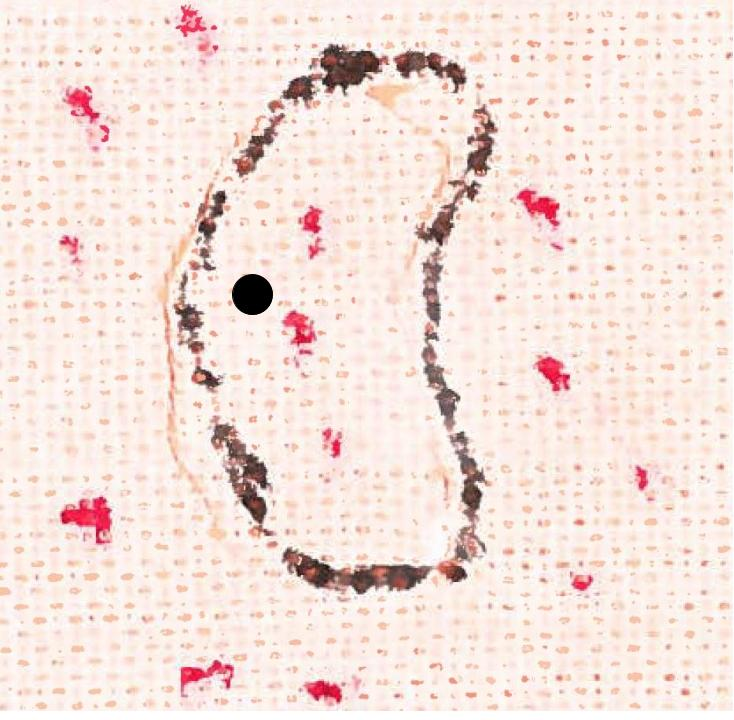
\includegraphics[height=1cm]{tps-experiments/shapes-robot/2-dot.jpg} &           \textbf{36.77 \%} \\
% 3 &   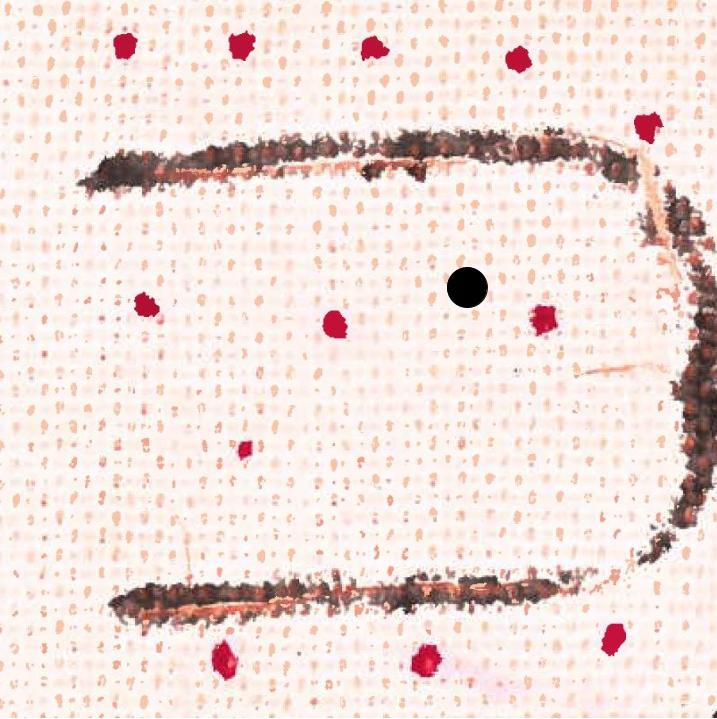
\includegraphics[height=1cm]{tps-experiments/shapes-robot/3-dot.jpg} &         \textbf{  75.33 \%}
% \\\rowcolor[HTML]{E0E0E0}
% 4 &   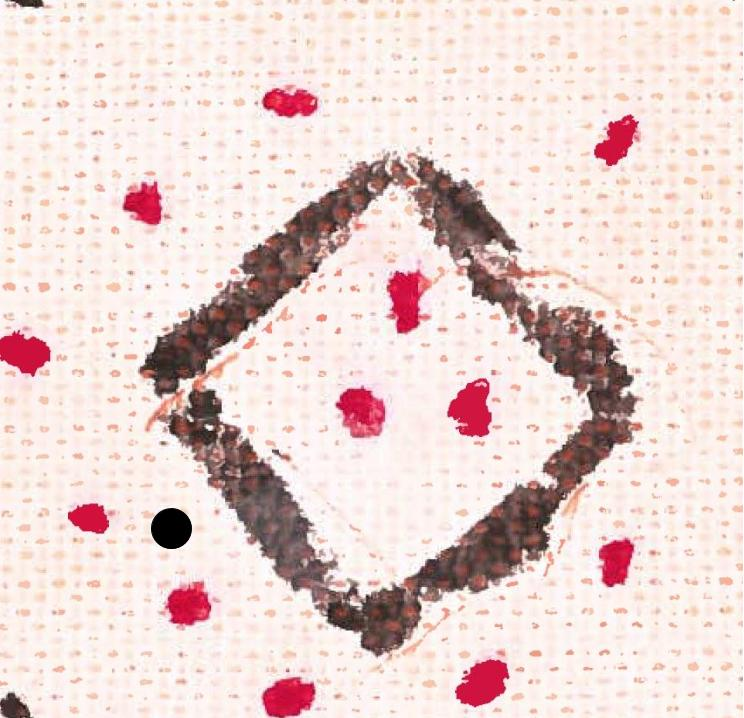
\includegraphics[height=1cm]{tps-experiments/shapes-robot/4-dot.jpg} &           -44.59 \% 
% \\
% \midrule
% % \hline 
% \rowcolor[HTML]{FFC72C}
% \bottomrule
% % \hline
% \end{tabular}
\begin{tabular}{cccc}
\hline
% \rowcolor[HTML]{CBCEFB}
%&Shape & Tensioning Method \\
%\rowcolor[HTML]{CBCEFB}
&  1 & 2 & 3 & 4 \\
\hline
 Shape \vspace{10pt} & 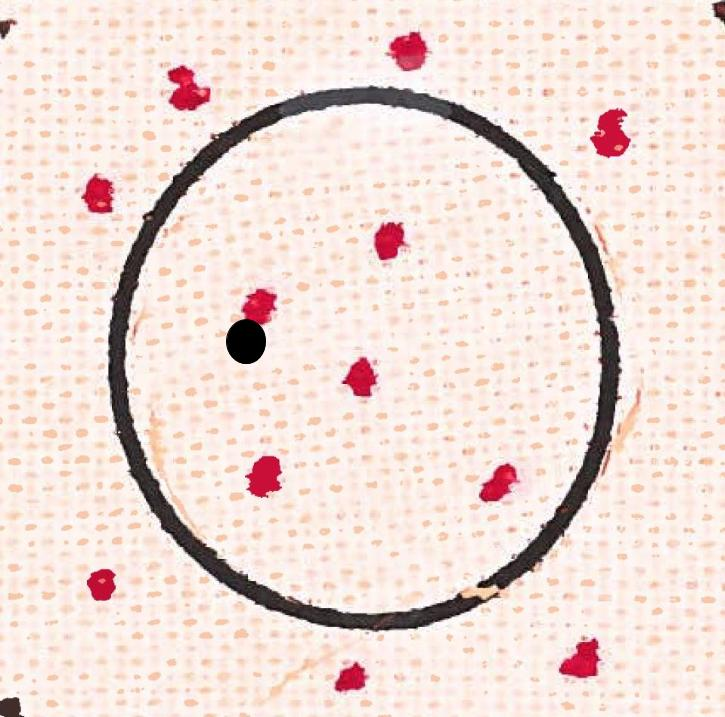
\includegraphics[height=1.2cm]{tps-experiments/shapes-robot/1-dot.jpg} & 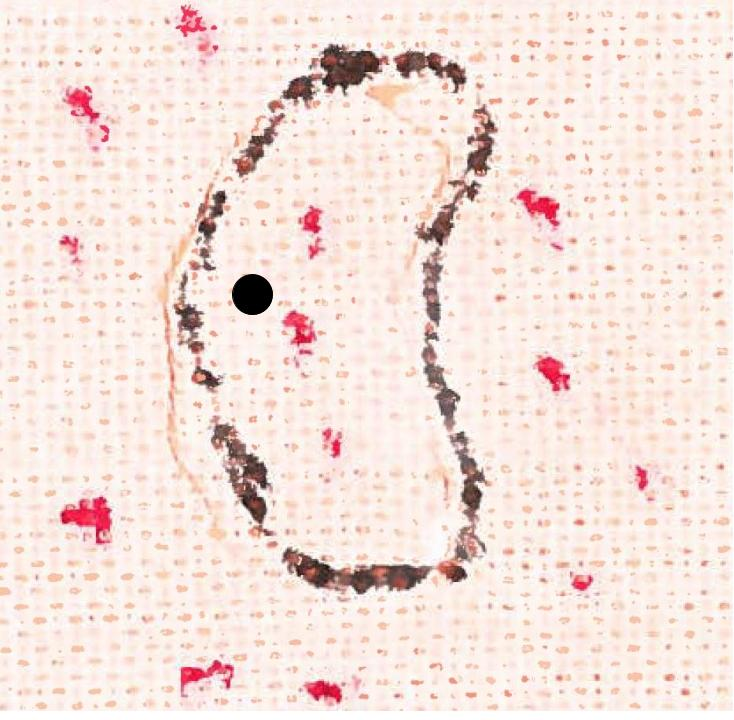
\includegraphics[height=1.2cm]{tps-experiments/shapes-robot/2-dot.jpg} &   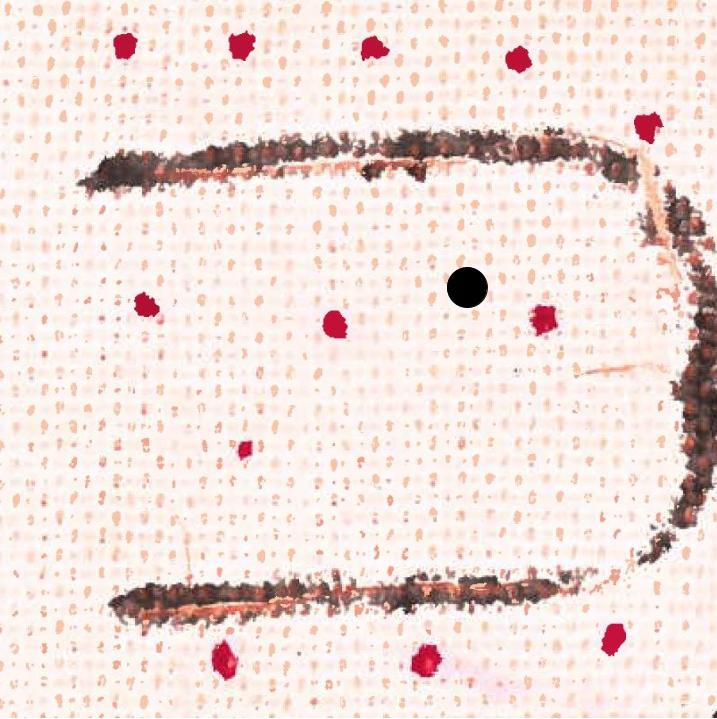
\includegraphics[height=1.2cm]{tps-experiments/shapes-robot/3-dot.jpg} & 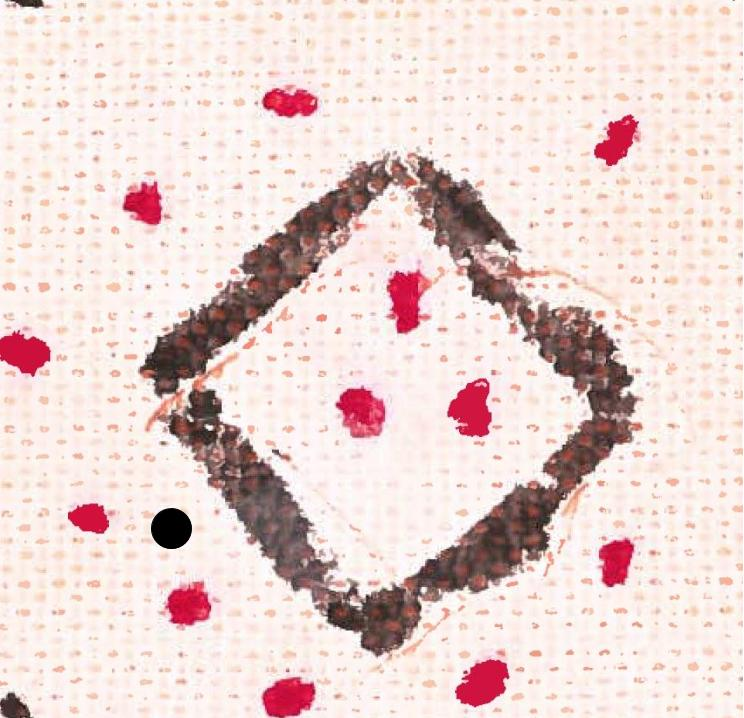
\includegraphics[height=1.2cm]{tps-experiments/shapes-robot/4-dot.jpg} \\
Deep RL & \textbf{118.63 \%}& \textbf{36.77 \%} & \textbf{  75.33 \%} &   -44.59 \\ 
% \bottomrule
% \midrule
% \midrule
% \hline 
% \rowcolor[HTML]{FFC72C}
\hline
% \hline
\end{tabular}
\vspace{-10pt}
\end{table}